\documentclass[a4paper,12pt]{book}
\usepackage{graphicx}
\usepackage[export]{adjustbox}
\usepackage{subcaption}
\graphicspath{{Pics/}}
\usepackage{charter}
\usepackage{fancyhdr}
\usepackage{enumerate}
\usepackage{enumitem}
\usepackage{siunitx}
\usepackage{amssymb}
\usepackage{longtable}
\usepackage{multicol}
\usepackage{multirow}
\usepackage{hhline}
\usepackage{parskip}
\setlength{\parskip}{6pt}
\usepackage{ragged2e}
\usepackage{geometry} %margin
\geometry{left=2.1cm,right=2.1cm,top=3cm,bottom=3cm}
\usepackage{setspace}
\SetSinglespace{1.2}
\singlespacing
\renewcommand{\ttfamily}{\fontfamily{pcr}\selectfont}
%\renewcommand{\familydefault}{\rmdefault}

\usepackage[,table]{xcolor}
\definecolor{LightBlue}{cmyk}{0.16,0.03,0.04,0}
\definecolor{Title}{cmyk}{0.8,0.1,0,0.3}
\setlength{\arrayrulewidth}{0.3mm}
\setlength{\tabcolsep}{2pt}
\setlength{\headheight}{15pt}
\renewcommand{\arraystretch}{1}
\usepackage{tikz}
\usepackage{nicematrix}
\newcommand*\circled[1]{\tikz[baseline=(char.base)]{\node[shape=circle,draw,inner sep=1pt] (char) {#1};}}

\newcolumntype{s}{>{\columncolor{Title}\RaggedLeft} m{3.5em}} % columntype for chapter title
\newcolumntype{d}{>{\columncolor{LightBlue}\RaggedRight} m{\textwidth}} % columntype for code bloc
\newcolumntype{a}{>{\columncolor{LightBlue}\RaggedRight} m{0.96\textwidth}} % columntype for secondary code bloc

\usepackage{titlesec}
\usepackage[hidelinks]{hyperref}
\urlstyle{same}

\captionsetup[figure]{labelsep=period,font={bf}}
\captionsetup[table]{font={bf},labelsep=period}

\newcommand{\titlename}{}

\newcommand{\chaptertitle}[2]{ %reset chapter format
\vspace{-120pt}
\gdef\titlename{#1}
{
\SetSinglespace{1.1}
\singlespacing
\Huge\bfseries
\setlength{\tabcolsep}{8pt}
\renewcommand{\arraystretch}{1.5}
\begin{tabular}{s >{\RaggedRight}m{14.5em}}
\textcolor{white}{Chapter\newline\thechapter}&\textcolor{Title}{#2}
\end{tabular}
}
}

\newcommand{\partpic}[1]{%insert picture
    \tikz[remember picture,overlay] \node at (current page.center){\includegraphics[width=\paperwidth]{#1}};
}

\titleformat{\part} %reset part %format
{\huge\bfseries} % format
{} % label
{0em} % sep
{\Centering} % before-code

\titleformat{\chapter} %reset chapter %format
{\huge\bfseries} % format
{} % label
{0em} % sep
{\Centering} % before-code
\titlespacing{\chapter}{0pt}{0pt}{0pt}

\titleformat{\section} %reset section %format
{\Large\bfseries} % format
{\textcolor{Title}{\thesection}} % label
{0.5em} % sep
{\color{Title}} % before-code
\titlespacing{\section}{0pt}{12pt}{6pt}

\titleformat{\subsection} %reset subsection %format
{\large\bfseries} % format
{\textcolor{Title}{\thesubsection}} % label
{0.5em} % sep
{\color{Title}} % before-code
\titlespacing{\subsection}{0pt}{8pt}{6pt}

\newenvironment{term}[1]{
    \textbf{#1}

    \leftskip 1em
    \parskip 0pt
}

\newenvironment{secterm}[1]{
    \textbf{#1}

    \leftskip 2em
    \parskip 0pt
}

\newenvironment{codebloc}{ %define code bloc style
    \ttfamily\footnotesize
    \renewcommand{\arraystretch}{1}
}

\newcommand{\note}[2][NOTE]{ %Note/Tips
\vspace{6pt}
\begin{tabular}{b{\textwidth}}
\hline
\fontfamily{phv}\selectfont \textbf{#1}\\
\leftskip 1em #2\\
\hline
\end{tabular}
}

\newcommand{\secnote}[2][NOTE]{ %Note/Tips
\vspace{6pt}
\begin{tabular}{b{0.93\textwidth}}
\hline
\fontfamily{phv}\selectfont \textbf{#1}\\
\leftskip 1em #2\\
\hline
\end{tabular}
}

\title{ESP32-C3 Wireless Adventure\par \Large A comprehensive guide to IoT}
\author{Espressif Systems}
\date{\today}

\pagestyle{fancy} % reset head&foot
\fancyhead{} % clear all header fields
\renewcommand\headrulewidth{0pt}
\fancyfoot{} % clear all footer fields

\begin{document}

{\makeatletter
\let\ps@plain\ps@empty
\makeatother
\part[Preparation]{\setcounter{page}{1}\partpic{Starting/1c}}
}

\fancyfoot[LE]{\fontfamily{cmss}\selectfont{\textbf{\thepage} \ \textit{ESP32-C3 Wireless Adventure: A comprehensive guide to IoT}}}
\fancyfoot[RO]{\fontfamily{cmss}\selectfont{\textit{Chapter \thechapter. \titlename} \ \textbf{\thepage}}}

\chapter[Introduction to IoT]{\chaptertitle{Introduction to IoT}{Introduction to IoT}}

\vspace{24pt}
At the end of the 20th century, with the rise of computer networks and communication technologies, Internet rapidly integrated into people's lives. As Internet technology continues to mature, the idea of Internet of Things (IoT) was born. Literally, IoT means an Internet where things are connected. While the original Internet breaks the limits of space and time and narrows the distance between “person and person”, IoT makes “things” an important participant, bringing “people” and “things” closer together. In the foreseeable future, IoT is set to become the driving force of the information industry.

So, what is the Internet of Things?

It is hard to accurately define the Internet of Things, as its meaning and scope are constantly evolving. In 1995, Bill Gates first brought up the idea of IoT in his book \textit{The Road Ahead}. Simply put, IoT enables objects to exchange information with each other through Internet. Its ultimate goal is to establish an “Internet of Everything”. This is an early interpretation of IoT, as well as a fantasy of future technology. Thirty years later, with the rapid development of economy and technology, the fantasy is coming into reality. From smart devices, smart homes, smart cities, Internet of Vehicles and wearable devices, to the “metaverse” supported by IoT technologies, new concepts are constantly emerging. In this chapter, we will begin with an explanation of the architecture of Internet of Things, and then introduce the most common IoT application, the smart home, in order to help you get a clear understanding of IoT.

\section{Architecture of IoT}

Internet of Things involves multiple technologies which have different application needs and forms in different industries. In order to sort out the structure, the key technologies and application characteristics of IoT, it is necessary to establish a unified architecture and a standard technical system. In this book, the architecture of IoT is simply divided into four layers: perception \& control layer, network layer, platform layer, and application layer.

\begin{term}{Perception \& Control Layer}
    As the most basic element of the IoT architecture, perception \& control layer is the core to realise the comprehensive sensing of IoT. Its main function is to collect, identify and control information. It consists of a variety of devices with the ability of perception, identification, control and execution, and is responsible for retrieving and analysing data such as material properties, behavioural trends, and device status. In this way, IoT gets to recognise the real physical world. Besides, the layer is also able to control the status of the device.

    \parskip 6pt
    The most common devices of this layer are various sensors, which play an important role in information collection and identification. Sensors are like human sensory organs, such as photosensitive sensors equalling to vision, acoustic sensors to hearing, gas sensors to smelling, and pressure- and temperature-sensitive sensors to touching. With all these “sensory organs”, objects become “alive” and capable of intelligent perception, recognition and manipulation of the physical world.
\end{term}

\begin{term}{Network Layer}
    The main function of the network layer is to transmit information, including data obtained from the perception \& control layer to specified target, as well as commands issued from the application layer back to the perception \& control layer. It serves as an important communication bridge connecting different layers of an IoT system. To set up a basic model of Inter\textbf{net} of Things, it involves two steps to integrate objects into a \textbf{net}work: access to Internet and transmission through Internet.
    
    \parskip 6pt
    \begin{secterm}{Access to Internet}
        Internet enables interconnection between person and person, but fails to include things into the big family. Before the advent of IoT, most things were not “network-able”. Thanks to the continuous development of technology, IoT manages to connect things to the Internet, thus realizing interconnection between “people and things”, and “things and things”. There are two common ways to implement Internet connection: wired network access and wireless network access.

        \parskip 6pt
        Wired network access methods include Ethernet, serial communication (e.g., RS-232, RS-485) and USB, while wireless network access depends on wireless communication, which can be further divided into short-range wireless communication and long-range wireless communication.
        
        Short-range wireless communication includes ZigBee, Bluetooth$^\circledR$, Wi-Fi, Near-Field Communication (NFC), and Radio Frequency Identification (RFID). Long-range wireless communication includes Enhanced Machine Type Communication (eMTC), LoRa, Narrow Band Internet of Things (NB-IoT), 2G, 3G, 4G, 5G, etc.
    \end{secterm}

    \begin{secterm}{Transmission through Internet}
    Different methods of Internet access lead to corresponding physical transmission link of data. The next thing is to decide which communication protocol to use to transmit the data. Compared with Internet terminals, most IoT terminals currently have fewer available resources, such as processing performance, storage capacity, network rate, etc., so it is necessary to choose a communication protocol that occupies fewer resources in IoT applications. There are two communication protocols that are widely used today: Message Queuing Telemetry Transport (MQTT) and Constrained Application Protocol (CoAP).
    \end{secterm}
\end{term}

\begin{term}{Platform Layer}
    The platform layer mainly refers to IoT cloud platforms. When all IoT terminals are networked, their data need to be aggregated on an IoT cloud platform to be calculated and stored. The platform layer mainly supports IoT applications in facilitating access and management of massive devices. It connects IoT terminals to the cloud platform, collects terminal data, and issues commands to terminals, so as to implement remote control. As an intermediate service to assign equipment to industry applications, the platform layer plays a connecting role in the entire IoT architecture, carrying abstract business logic and standardized core data model, which can not only realize rapid access of devices, but also provide powerful modular capabilities to meet various needs in industry application scenarios. The platform layer mainly includes functional modules such as device access, device management, security management, message communication, monitoring operation and maintenance, and data applications.

    \parskip 6pt
    \begin{itemize}
        \item Device access, realising the connection and communication between terminals and IoT cloud platforms.
        \parskip 0pt
        \item Device management, including functions such as device creation, device maintenance, data conversion, data synchronization, and device distribution.
        \item Security management, ensuring the security of IoT data transmission from the perspectives of security authentication and communication security.
        \item Message communication, including three transmission directions, that is, the terminal sends data to the IoT cloud platform, the IoT cloud platform sends data to the server side or other IoT cloud platforms, and the server side remotely controls IoT devices.
        \item Monitoring O\&M, involving monitoring and diagnosis, firmware upgrade, online debugging, log services, etc.
        \item Data applications, involving the storage, analysis and application of data.
    \end{itemize}
\end{term}

\begin{term}{Application Layer}
    The application layer uses the data from the platform layer to manage the application, filtering and processing them with tools such as databases and analysis software. The resulting data can be used for real-world IoT applications such as smart healthcare, smart agriculture, smart homes, and smart cities.
\end{term}

Of course, the architecture of IoT can be subdivided into more layers, but no matter how many layers it consists of, the underlying principle remains essentially the same. Learning about the architecture of IoT helps deepen our understanding of IoT technologies and build fully functional IoT projects.

\section{IoT Application in Smart Homes}
IoT has penetrated into all walks of life, and the most closely related IoT application to us is the smart home. Many traditional appliances are now equipped with one or more IoT devices, and many newly built houses are designed with IoT technologies from the start. Figure \ref{Common smart home devices} shows some common smart home devices.

\begin{figure}[!ht]
    \centering
    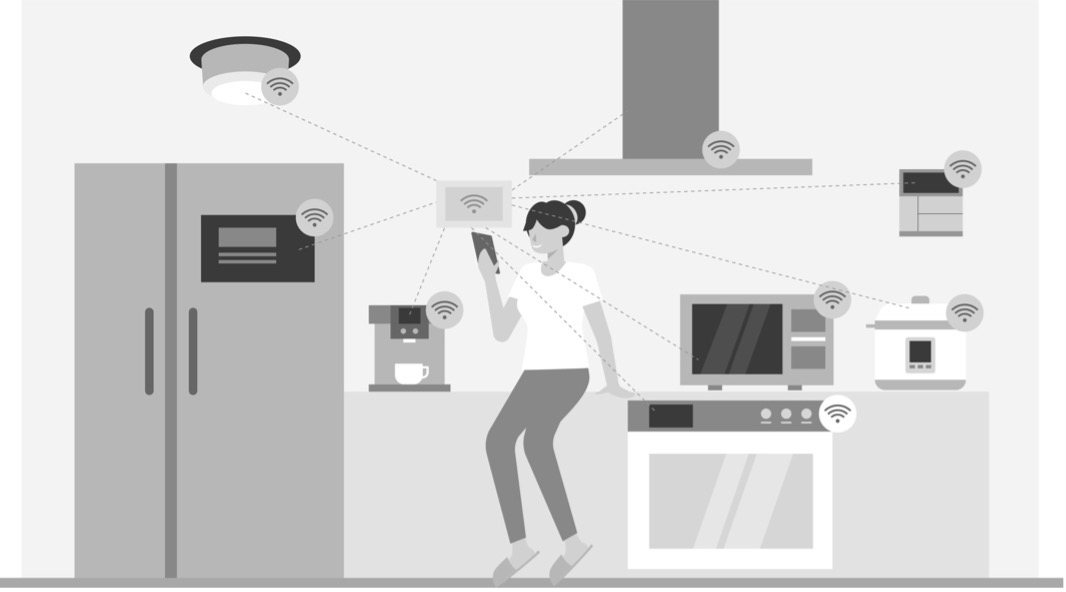
\includegraphics[width=0.75\textwidth]{D1Z/1-1}
    \caption{Common smart home devices}
    \label{Common smart home devices}
\end{figure}

The development of smart home can be simply divided into smart product stage, scene interconnection stage and intelligent stage, as shown in Figure 1.2.

\begin{figure}[!ht]
    \centering
    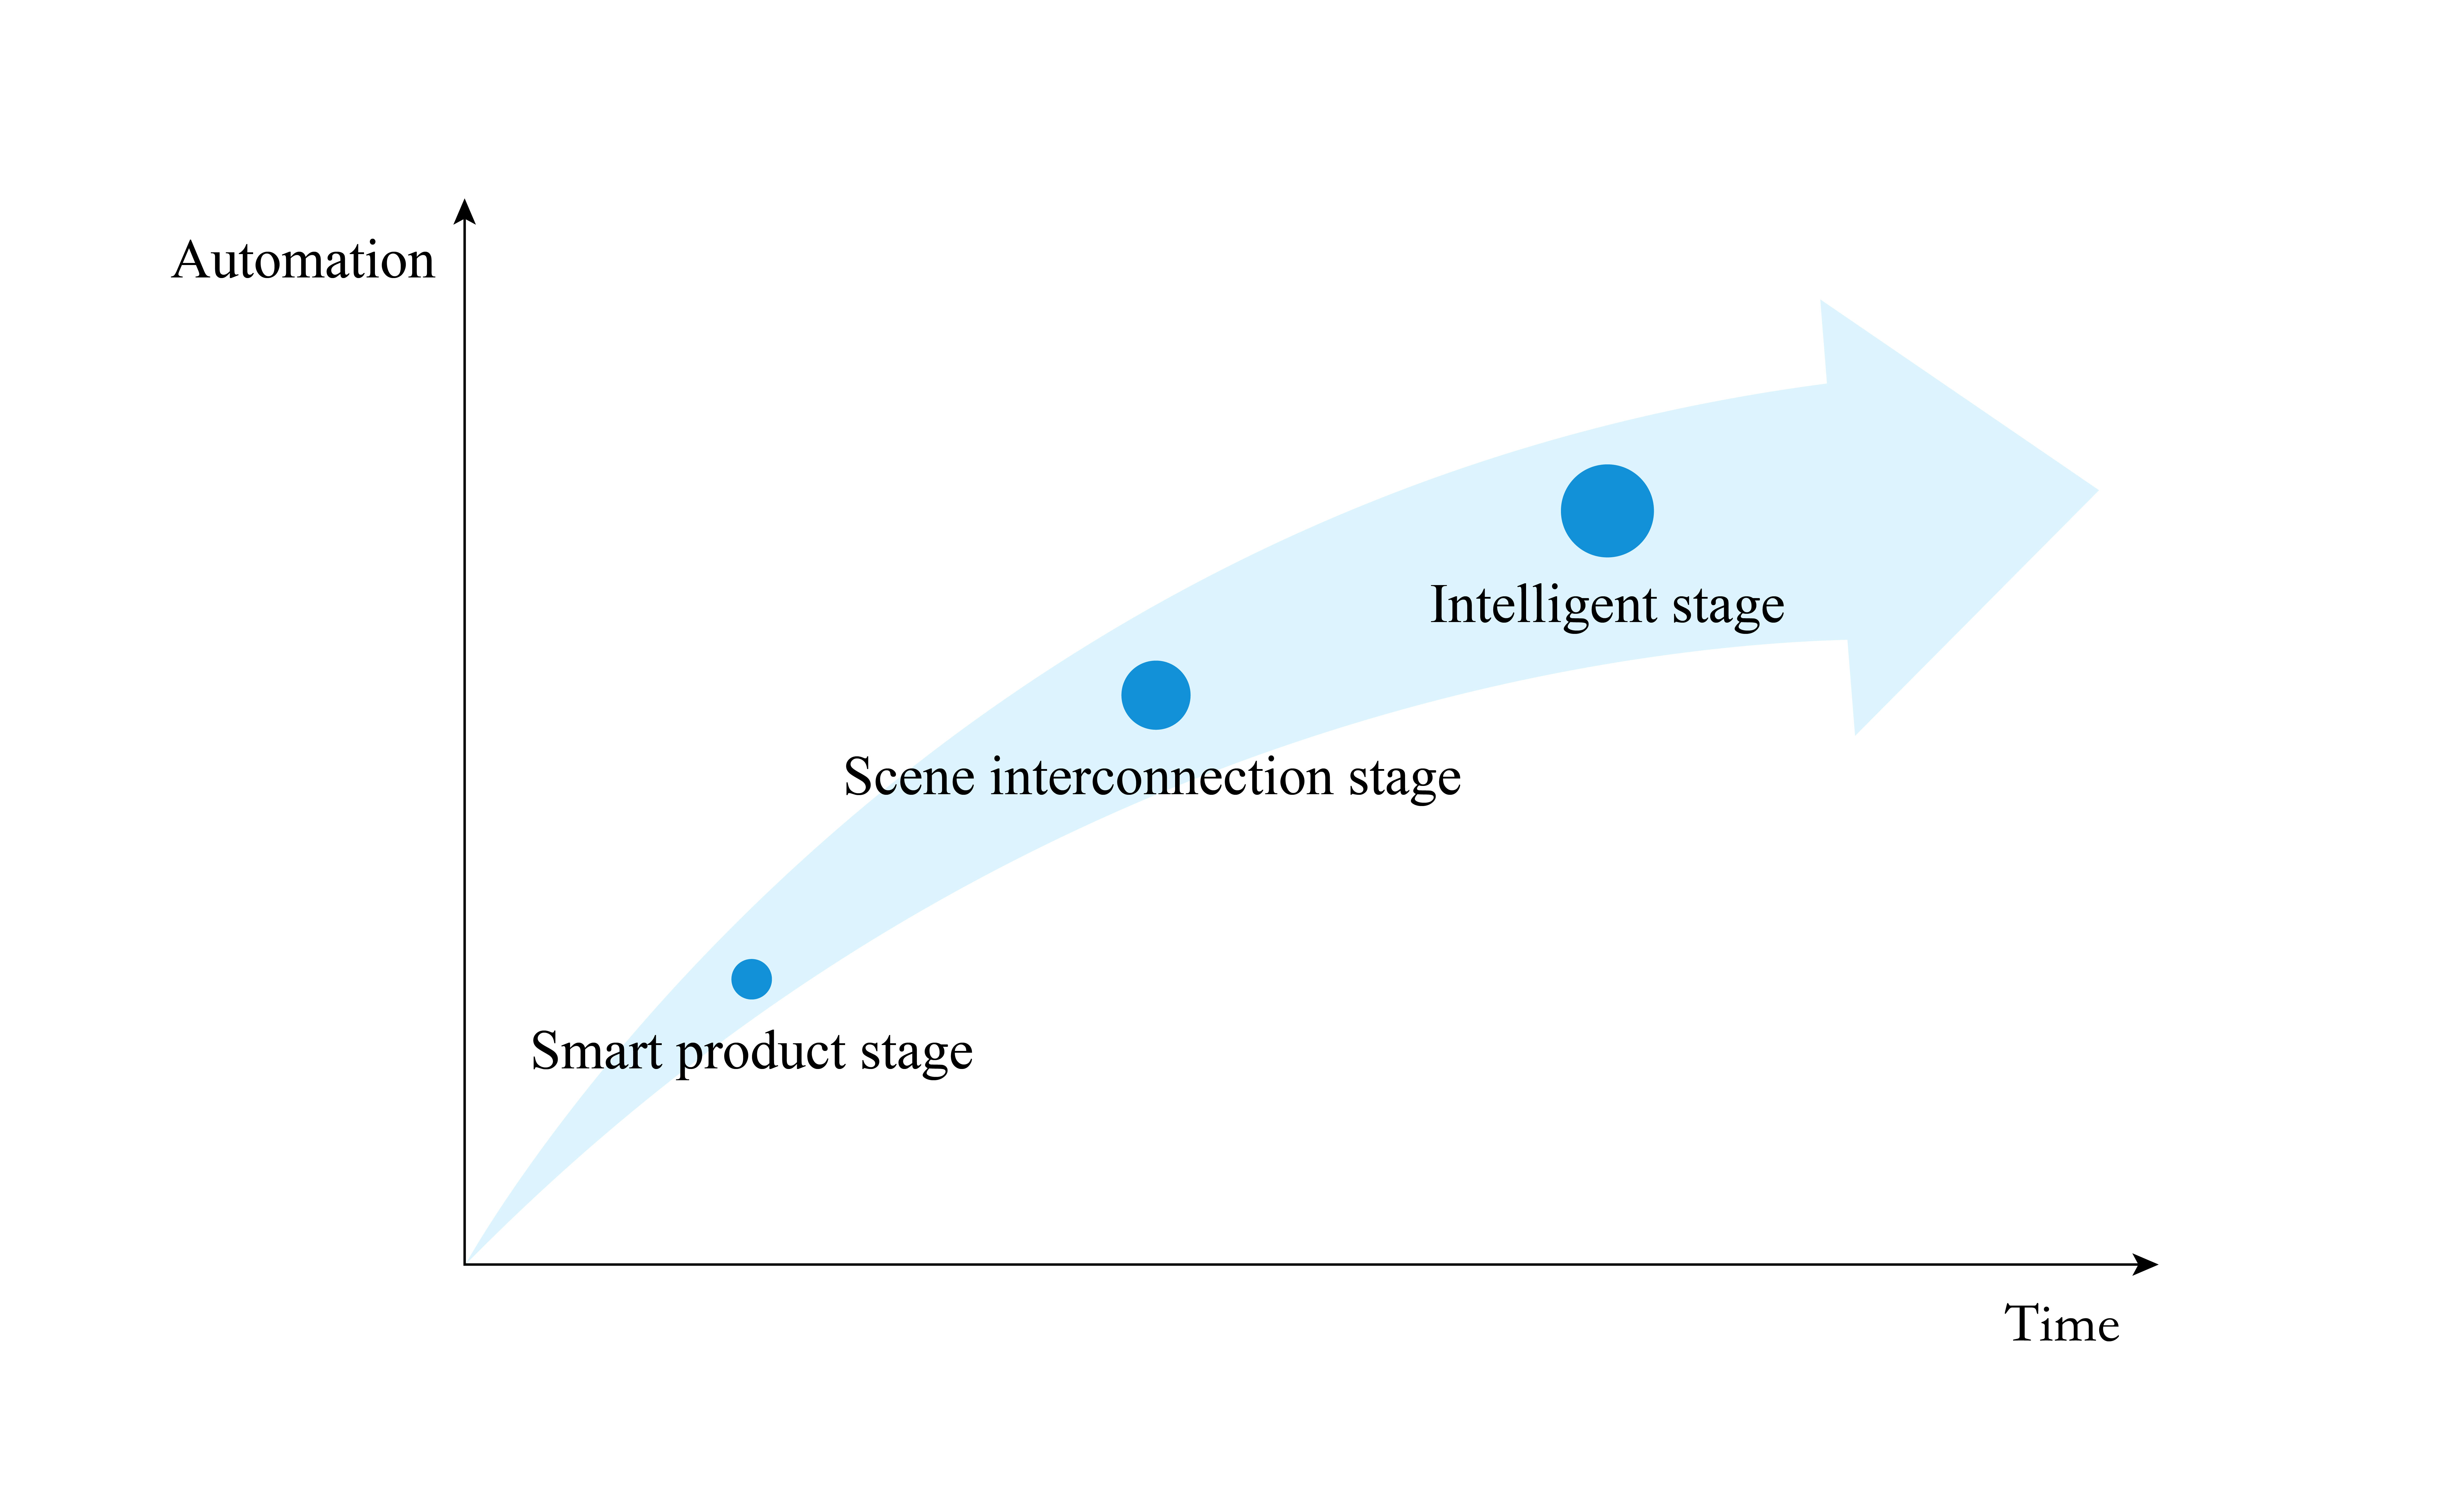
\includegraphics[width=0.8\textwidth]{D1Z/1-2}
    \caption{Development stage of smart home}
\end{figure}

The first stage is about \textbf{smart products}. Different from traditional homes, in smart homes, IoT devices receive signals with sensors, and are networked through wireless communication technologies such as Wi-Fi, Bluetooth LE, and ZigBee. Users can control smart products in a variety of ways, such as smartphone apps, voice assistants, smart speaker control, etc.

The second stage focuses on \textbf{scene interconnection}. In this stage, developers are no longer considering controlling single smart product, but interconnecting two or more smart products, automating to a certain extent, and finally forming a custom scene mode. For example, when the user presses any scene mode button, the lights, curtains, and air conditioners will be automatically adapted to the presets. Of course, there is the prerequisite that the linkage logic are readily set up, including trigger conditions and execution actions. Imagine that the air conditioning heating mode is triggered when the indoor temperature drops below 10°C; that at 7 o’clock in the morning, music is played to wake up the user, smart curtains are opened, and the rice cooker or bread toaster starts through a smart socket; as the user gets up and finishes washing, breakfast is already served, so that there will be no delay in going to work. How convenient has our life become!

The third stage goes to \textbf{intelligence stage}. As more smart home devices are accessed, so will the types of data generated. With the help of cloud computing, big data and artificial intelligence, it is like a “smarter brain” has been planted into smart homes, which no longer require frequent commands from the user. They collect data from previous interactions and learn the user's behaviour patterns and preferences, so as to automate activities, including providing recommendations for decision-making.

Currently, most smart homes are at the scene interconnection stage. As the penetration rate and intelligence of smart products increase, barriers between communication protocols are being removed. In the future, smart homes are bound to become really “smart”, just like the AI system Jarvis in \textit{Iron Man}, which can not only help the user control various devices, handle daily affairs, but also have super computing power and thinking ability. In the intelligent stage, human beings will receive better services both in quantity and quality.

\end{document}